%Methode: paarweiser Vergleic
%~ Um die in Frage stehenden Blockchain-Implementierungen miteinander vergleichen zu können,
%~ soll den eigenen Kriterien jeweils ein von der Software unabhängiges Gewicht als Präferenz für die Wichtigkeit zugeordnet werden.

%~ Spezifisch für jedes Kriterien 

Der Vergleich der gewonnen Kriterien soll nicht nur der Entscheidungsfindung dienen, sondern auch der Kommunikation der Entscheidung.
%~ Komplexität ist hier ein Gegenpol zur Nachvollziehbarkeit.
Nicht nur um sie nachvollziehbar zu machen, sondern auch weil im Zweifel mehrere Entscheider Einfluss nehmen möchten.
Daher steht die Frage der Darstellung hier im Vordergrund der Kommunikation.

Eine Wertung in Zahlen macht die Vergleichbarkeit einfacher.
Die Zuordnung von Attributen zur Abstufung nicht-binärer Bewertungen ist der Kommunikation zuträglich.
Da die einzelnen Kriterien in unterschiedliche -- weitgehend atomare -- Aspekte zerfallen kann auch eine Akkumulation für die quantitative Gesamtbewertung für ein Kriterium erfolgen.
%~ \footnote{ \autocite{p:vergleich}}


\section{Optionen zur Darstellung}\label{depiction}

Entscheidungsprozesse müssen nicht nur innerhalb einer \gls{BC} nachvollziehbar sein.
Gerade in Unternehmen ist die Dokumentation und ggf. Wiederholbarkeit -- z.B. im Rahmen des betrieblichen Benchmarking -- von gesteigertem Wert für den dauerhaften wirtschaftlichen Erfolg über den Einsatzzeitraum eines IT-Systems hinaus.

\subsection{Checklisten}

Eine sehr einfache und vielfältig gestaltbare Möglichkeit stellen Checklisten dar.
Sie kann zur Überprüfung von binären Kriterien kann sehr einfach im Sinne von erfüllt/nicht erfüllt \enquote{abgehakt} werden.

%~ die eigenschaft btf oder nicht und in klassen 2/3 oder 1/2
Wenn das Kriterium Konsens auf die für den Anwendungsfall notwendigen seiner Aspekte reduziert wird kann somit schnell ein Vergleich erfolgen welche \gls{BCI} das Kriterium besser/schlechter/gleich erfüllt.\footnote{\cite{TN_libero_mab215408815}}

%~ \textbf{Beispielhaft eine Checkliste für das Kriterium \namref{krit:consensus} (\ref{krit:consensus})}
\begin{itemize}
\item Finalität
\item \gls{BFT}
\item Austauschbarkeit
\item Erlaubnisfreiheit
\item Dezentralität
\end{itemize}

Diese Darstellung eignet sich nicht für komplexere, multikriterielle Vergleiche.
Allein die Länge der Checkliste macht die Bewertung schnell unübersichtlich und eignen sich daher eher für die Unterstützung der Abarbeitung eines Vorgangs denn für die Entscheidungsfindung.

\subsection{Entscheidungsquadrat}

Eine Darstellung im Entscheidungsquadrat erschöpft sich bereits bei zwei Dimensionen, eine dritte erweitert bereits zum Würfel und führt zu einer schlechteren Ablesbarkeit.
Häufig werden die Dimensionen \enquote{dringlich} und \enquote{wichtig} verwendet; also eine Entscheidung zur Priorisierung unterstützt.
%~ Um die Entscheidungsstruktur in Unternehmen besser abzubilden, werden die Faktoren umgewidmet auf Preis und Relevanz.
Damit eignet sich das Entscheidungsquadrat in dieser Form z.B. zur Unterstützung hinsichtlich geplanter aber noch nicht verfügbarer Eigenschaften einer \gls{BCI}.
%~ Dabei wird der Zeitfaktor 

\subsection{Ranking}\label{dep:ranking}

Die Wertungen werden in einer Dimension auf- oder absteigend geordnet. Eventuelle gleiche Wertungen können auftreten, sodass keine eindeutige Reihenfolge zustande kommt.
Die einfache Bewertung ohne Attributen oder Zahlen kann mit einer Rangfolge zum Ausdruck gebracht werden; d.h. eine Quantifizierung in Zahlen ist nicht unbedingt notwendig.
Im umgekehrten Fall, der Darstellung einer bereits erfolgten Bewertung mit Zahlen oder auch in ihrem Rang definierten Attributen ist lediglich noch eine verdeutlichende Wirkung zu erwarten.

Sofern eine quantitative Gesamtbewertung vorliegt, eignet sich das Ranking für die Darstellung der naheliegendsten \gls{BCI}.
Die Erstellung ist aber schwer nachvollziehbar und deshalb auch hinsichtlich der Wiederholbarkeit fehleranfällig.

\subsection{Paarweiser Vergleich}\label{dep:pugh}

Der Paarweise Vergleich (auch Pugh~Matrix) ermöglicht einen strukturierten Vergleich für eine beliebige Anzahl von Parametern.
Dabei werden die Kriterien horizontal und vertikal in eine Tabelle (Abb.\,\ref{abb:pugh-matrix}) eingetragen.
Die horizontale Addition der Wertungen kann als eine Rangwertung genutzt werden.\footnote{\cite{TN_libero_mab21000123709}}

\begin{figure}[!htp]
\centering
\begin{tabular}{|r||r|r|r|r|r|r||r|}
\hline
\(K_i\)	& 0 	& 1 	& 2 	& 3 	& 4 	& 5	& \(\sum{}\)\\
\hline \hline
0		& --	& 0		& 1		& 2		& 0		& 1	& 4			\\
\hline
1		& 2		& --	& 0		& 1		& 2		& 0	& 5			\\
\hline
2		& 1		& 2		& --	& 1		& 2		& 0	& 6			\\
\hline
3		& 0		& 1		& 1		& --	& 1		& 2	& 5			\\
\hline
4		& 2		& 0		& 0		& 1		& --	& 0	& 3			\\
\hline
5		& 1		& 2		& 2		& 0		& 2		& --& 7			\\
\hline \hline
\(\sum{}\) & \multicolumn{6}{r||}{} & {30} \\
\hline
\end{tabular}
\captionof{figure}[Beispiel Pugh Matrix]{\label{abb:pugh-matrix} Beispiel Paarweiser Vergleich der Kriterien}
\end{figure}

Die Zellen werden nun mit den Wertungen bis zu einem Maximum \(m \ge 2\) aus der Menge von Wertungsmöglichkeiten \(M\) für den direkten Vergleich von zwei sich kreuzenden Kriterien befüllt.
Dazu wird eine Zahl \(w \in [0;m] \)  höher für eine stärkere Wertung des Kriteriums in der Zeile vergeben, und geringer für eine stärkere Wertung des Kriteriums in der Spalte.
Die Diagonale in der das gleiche Kriterium mit sich selbst verglichen würde, entfällt und alle Vergleiche unterhalb der Diagonale sind invers zu den oberen Werten und können schlicht als \(w' = m - w\) am Maximalwert \(m\) gespiegelt werden.
Um eine neutrale Wertungen zum Ausdruck bringen zu können, muss die Menge \(M\) eine ungerade Anzahl an Möglichkeiten für \(w\) vorgeben.

Auch die Beteiligung mehrerer Entscheider ist die Kombination durch ein Produkt der einzelnen Bewertungen mehrstufig umsetzbar.
Eine Unterstützung durch z.B. eine Tabellenkalkulation ist machbar, aber mit manuellen Aufwand für Anpassungen verbunden.
Jeder einzelne Bewertungsvorgang bleibt aufwändig -- und der Aufwand steigt exponentiell mit der Anzahl der Kriterien.
Damit ist das Bewertungsverfahren nicht gut geeignet in einem Meeting mit überschaubarem Zeitrahmen durchgeführt zu werden.

\subsection{Netzdiagramm}\label{dep:web}

Das Netzdiagramm (auch Radardiagramm, Kiviat-Diagramm, oder Sterndiagramm) besteht aus mindestens drei unabhängigen Parametern als Strahlen (für die quantitative Wertung der Kriterien) ausgehend von einem gemeinsamen Mittelpunkt in einer Darstellung (Abb.\,\ref{disp:web:pic}).

\begin{figure}[!htp]
%~ \scalegraphics{img/disp-web}
\centering
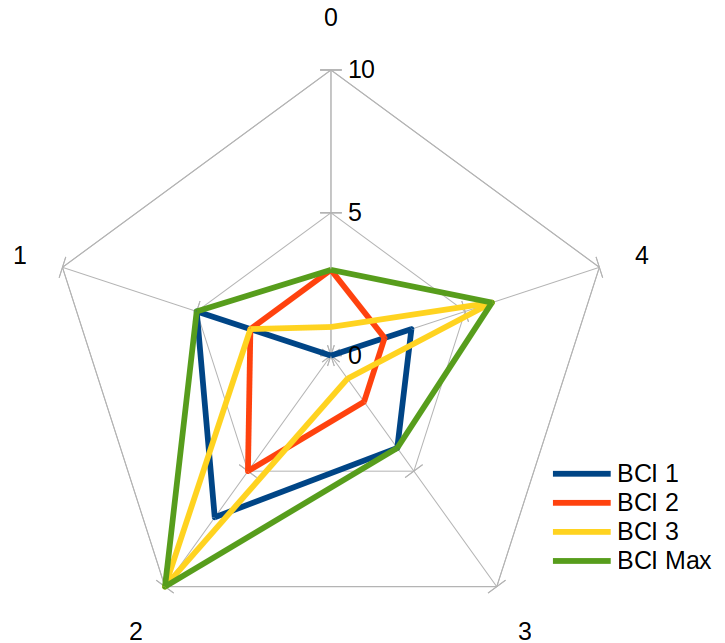
\includegraphics[width=.6\textwidth]{img/disp-web}
\captionof{figure}[Beispiel Netzdiagramm]{\label{disp:web:pic} Beispiel Netzdiagramm}
\end{figure}

Abhängig vom Radius der Abbildung lässt sich so leicht eine zweistellige Anzahl von Parametern einbringen;
optimal ist die Darstellung jedoch eher für 5-7 Kriterien.
Eine mehrdimensionale Darstellung wie das Netzdiagramm eignet sich um die Parameter einer \gls{BCI} in einer Abbildung zusammenzufassen.
%~ Sowohl Gegensätze als auch Skalierungen können so verdeutlicht werden.
Die Fläche des Vieleckes, dass sich aus den am je abgezeichneten Strahlen verbundenen Schnittpunkten ergibt, steht sowohl mit ihrem Betrag als auch dem optischen Eindruck für die Bewertung der damit illustrierten \gls{BCI}.
Für die Darstellung und auch Berechnung ist eine gleichwinklige Verteilung der Strahlen hilfreich.

Die exakte Erstellung ist manuell nicht trivial; dank der simplen geometrischen Regeln aber leicht mit u.a. einer Tabellenkalkulation zu realisieren.
Soweit die Wertreihe für unterschiedliche \gls{BCI} voneinander abweichen, lassen sich auch zwei oder mehr Wertreihen in einer Abbildung zusammen fassen.

Unabhängig von der grafischen Erstellung kann die Berechnung vorgenommen werden.
Die Fläche \(F\) zerfällt in Dreiecke um den Mittelpunkt \(C\) bei denen jeweils die Seiten \(a, b\) und der Winkeln \(\gamma\) bekannt sind.

\[
F_{\text{Dreieck}} = \frac{ab\sin{\gamma}}{2}
\text{\hspace{2em}}\Rightarrow{}\text{\hspace{2em}}
F_{n\text{-Eck}} = \sum_{i=0}^{n} \frac{a_{i} b_{(i+1)\mod n} \sin{\gamma}}{2}
\]

Da die Winkel im gleichwinkligen \(n\)-Eck mit %\(\gamma\) für
\( \frac{\tau}{n}\ = \frac{2\pi}{n}\) bzw. \(\frac{360^\circ{}}{n}\) konstant sind,
kann die Berechnung der Entscheidungsgrundlage \(E\) für jeden Sektor vereinfacht werden.
Die Summe ist unter Beachtung der Grenzen dann ebenfalls leichter zu ermitteln.

\[
E_{\text{Sektor}} = ab 
\text{\hspace{2em}}\Rightarrow{}\text{\hspace{2em}}
E_{gesamt} = \sum_{i=0}^{n} a_{i} b_{(i+1)\mod n}\text{\hspace{3em}}\Big|{\gamma \text{ konstant}}
\]

Da der exakte Wert der Fläche nicht relevant ist, sondern das Verhältnis zu einem theoretischen Pareto Optimum,
kann dieses durch die Maximalwerte alle betrachteten \gls{BCI} gebildet werden.
Die einzelnen -- im Grunde wegen der Nichtaustauschbarkeit zwischen den \gls{BCI} -- nicht miteinander vergleichbaren
Kandidaten können jedoch über das Verhältnis mit dem Pareto Optimum miteinander verglichen werden.


%~ \section{Anwendung auf die Kriterien}

\section{Quantifizierung}

Die Quantifizierung -- also Bewertung in Zahlen -- der bisher durch Beschreibung (in Worten) durchgeführten subjektiven Bewertung soll das Verständnis für die Wertigkeit klarer zum Ausdruck bringen und ggf. eine Berechnung ermöglichen.
In jede Fall kann dadurch eine objektivere Sicht bzw. die Begründung für Anpassungen eingebracht werden.

%~ Als Beispiel dient hier die Bewertung 

\subsection{Gruppierung}

In der Wertung haben manche Kriterien eine höhere Priorität als andere.
Die Gruppierung ermöglicht die Konzentration auf diese Prioritäten und thematische Zusammenhänge.
%~ An dieser Stelle können die unterschiedlichen Wertebereiche auch gezielt mit einem weiteren Faktor ausgeglichen werden.

Die Einteilung kann genutzt werden um Schwerpunkte für den eigenen Anwendungsfall zu setzen,
%~ \begin{enumerate}
einzelne Kriterien hinsichtlich der Wertung an- oder abzuwählen und sich auf die für eigene Zwecke notwendigen Gruppen zu konzentrieren.
Die Einteilung sollte für den Bewertungsprozess z.B. dadurch hilfreich sein, dass unterschiedliche Spezialisten eine Teilentscheidung beitragen können.
Die Kriterien wurden beispielhaft in den drei Gruppen \nameref{krit:it} (\ref{krit:it}), \nameref{krit:blockchainproperties} (\ref{krit:blockchainproperties}) und \nameref{krit:oeconomics} (\ref{krit:oeconomics}), zusammengefasst.
%~ \end{enumerate}

\subsection{Klassifizierung}\label{classification}

Die in Worte gefasste Einteilung kann entlang des Wertungsgefälles mit Zahlen belegt werden.
Die einfachste Art von Klassen definieren sich durch Grenzen.
Jedoch ist der Übergang nicht immer eindeutig abgestuft.
Um das Problem handhabbar zu machen, wird vorgeschlagen die Unterteilung in binär beantwortbare Aspekte vorzunehmen.
Diese sollten mindestens so weit erweitert werden, wie es für die eigenen Zwecke notwendig ist.
Optimal wäre eine Erweiterung um Bedingungen bis die zu vergleichenden Kandidaten unterscheidbar werden.
Eine darüber hinausgehende Unterscheidung bedeutet lediglich mehr Arbeit in der Auswertung ohne einen direkten Nutzen; kann aber für eine künftige Iteration als vorbereitende Maßnahme wichtig sein.

Als Beispiel hierfür sei die Klassifizierung von Software-Lizenzen (s.a. \ref{krit:opensource}) angeführt.
Die Aspekte könnten sein:

%~ \begin{itemize}
%~ \item Verwendungserlaubnis ohne Einschränkungen
%~ \item Lesen der Quellen ohne Vorbedingunen
%~ \item Verteilen von Kopien
%~ \item 
%~ \end{itemize}

\begin{enumerate} 		\setlength\itemsep{0em}\setlength\parskip{0em}\setlength\topsep{0em}\setlength\partopsep{0em}\setlength\parsep{0em}
\item Open~Source gem. OSI (vgl. \ref{krit:opensource})
\item Behandlung von Software-Patenten
\item Gleiche Garantien auch ohne Auslieferung einer Software (z.B. Webservice)
\item Veränderung ist trotz \gls{DRM} garantiert
\end{enumerate}

Damit lassen sich die Lizenzen der behandelten Kandidaten in Wertungen 0/1 (nein/ja) unterscheiden.

\begin{figure}[!htp]
\centering
\begin{tabular}{l|lll}
Aspekt	& LGPL\,3.0 	& Apache~License\,2.0 & AGPL\,3.0 \\
\hline
\hline
1 		& 1	& 1	& 1	\\
\hline
2 		& 1	& 1	& 1	\\
\hline
3 		& 0	& 0	& 1	\\
\hline
4		& 1 & 0 & 0 \\
\hline
\hline
\(\sum\)& 3 & 2 & 3 \\
\end{tabular}
\captionof{figure}[Beispiel Wertung Softwarelizenzen]{\label{abb:wertung:oss} Beispiel einfache Wertung von Softwarelizenzen}
\end{figure}

\subsection{Gewichtung}

Das gleiche Ergebnis (\nameref{classification}, Abb.\,\ref{abb:wertung:oss}) für die LGPL\,3.0 und die AGPL\,3.0 in der Summe verdeutlicht,
dass vollständiger Unterscheidbarkeit das Ergebnis nicht eindeutig sein muss.

Um das Problem zu verringern, ist eine Gewichtung hilfreich.

\subsubsection*{Begründung am Beispiel}
Wir gewichten hier die Aspekte 2-4 höher weil sie für die unternehmerische Nutzung von gesteigerter Bedeutung sind.
Aspekt 1 wird nicht höher gewichtet, da es sich um das im technologischen Umfeld übliche Mindestmaß handelt, das auch eingehalten wird.
Wegen des primären Einsatzes von Webtechnologien und der daraus resultierenden Verwendung von Services in Netzwerken bei gleichzeitiger Kommplung mit der \gls{BCT}, die selbst auf Netzwerken basiert, wird Aspekt 3 nochmals stärker gewichtet.

\begin{figure}[!htp]
\centering
\begin{tabular}{l|llll}
Aspekt	& Gewichtung & LGPL\,3.0 	& Apache~License\,2.0 & AGPL\,3.0 \\
\hline
\hline
1 		& 1	& 1	& 1	& 1	\\
\hline
2 		& 2	& 2	& 2	& 2	\\
\hline
3 		& 3	& 0	& 0	& 3	\\
\hline
4		& 2	& 2 & 0 & 0 \\
\hline
\hline
\(\sum\)& --& 5 & 3 & 6 \\
\end{tabular}
\captionof{figure}[Beispiel Gewichtete Wertung]{\label{abb:wertung:oss2} Beispiel Gewichtete Wertung von Softwarelizenzen}
\end{figure}

Durch die Stärkere Gewichtung der möglicherweise geschäftskritischeren Fragen kann damit ein eindeutiges Ergebnis für das Kriterium ermittelt werden.
Wichtig für die Nachvollziehbarkeit ist die Dokumentation des Grundes für eine Gewichtung.

\subsection{Entscheidungsunterstützung}

Das verkürzte Beispiel zu den Software (Abb.\,\ref{abb:wertung:oss2}) lässt sich nun einfach per \nameref{dep:ranking} (\ref{dep:ranking}) entscheiden.
Der Nutzen der Abbildung nur eines Kriteriums ist jedoch sehr begrenzt.

Da Entscheidungen sehr leicht subjektiv werden sind die Maßnahmen zur Gruppierung, \nameref{classification} und Gewichtung entscheidend um
eine objektive und nachvollziehnbare Grundlage zu erreichen.

Der Paarweise Vergleich (\ref{dep:pugh}) kann mehrstufig eingesetzt zu einer guten Entscheidungsgrundlage führen.
Der mit Anzahl der Kriterien wachsende Aufwand und die geringe Eignung für die direkte bildliche Darstellung begrenzen den praktischen Nutzen.

Dagegen kann durch das \nameref{dep:web} (\ref{dep:web}) eine gute grafische Darstellbarkeit -- für sogar mehrere Kandidaten -- in einem Bild aufweisen.
Zusätzlich ist die Berechenbarkeit eines Entscheidungskriteriums und die Vergleichbarkeit mit einem Pareto-Optimum ein entscheidender Vorteil sowohl was die Einschränkungen für Präsentationen bei Entscheidern betrifft als auch die Argumentation bezüglich des theoretisch erreichbaren.
